\section{Deployment View}
\label{sec: deployment_view}%
The distribution of components capturing the topology of the system is illustrated below by using a deployment diagram.
The system is structured in a multitier architecture.
\newline
\begin{figure} [H]
    \begin{center}
        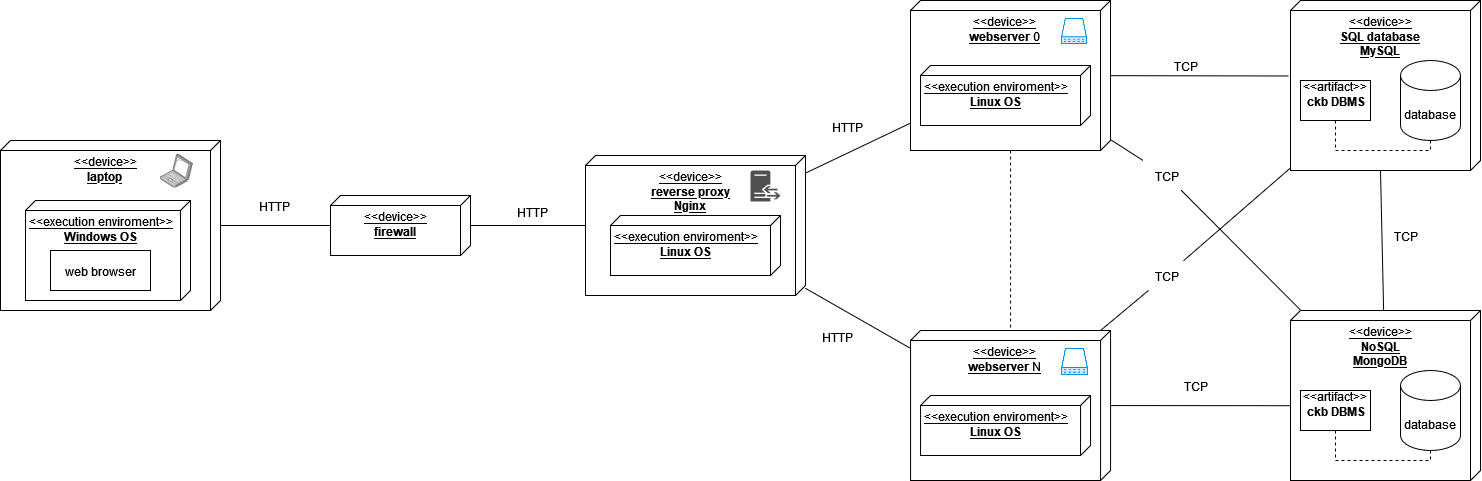
\includegraphics[width=1\linewidth]{Images/deployment_diag.png}
        \caption{Deployment diagram of the CKB platform.}
        \label{fig: depl_diagram}
    \end{center}
\end{figure}


\noindent\textbf{Laptop devices}\newline
This node represents a user's laptop, which is the client-side hardware. The "Windows OS" indicates that the laptop is running on the Windows operating system. 
The "web browser" is the software application used to access the web interface of the platform.

\noindent\textbf{Firewall}\newline
This is a security device that monitors and filters incoming and outgoing network traffic based on an organization's previously established security policies. 
Here, it acts as a barrier between secure internal networks and untrusted external networks, such as the internet.

\noindent\textbf{Reverse Proxy}\newline
This server is running Nginx, which is a web server that can also be used as a reverse proxy. This means it can distribute traffic to various servers, 
thereby acting as an additional layer of abstraction and control to smooth the flow of network traffic between clients and services.

\noindent\textbf{Webserver 0}\newline
This is one of potentially multiple web servers that handle the incoming HTTP requests from the client's web browser, process those requests, 
and serve the appropriate web pages. It runs on a Linux operating system, which suggests a preference for open-source solutions.

\noindent\textbf{Webserver N}\newline
This indicates there are multiple webservers in this deployment, following a similar configuration to "Webserver 0." 
The "N" represents an indefinite number, showing that the architecture is scalable and can include as many webservers as needed.

\noindent\textbf{SQL database (MySQL)}\newline
This database node uses MySQL, which is a relational database management system (RDBMS) based on SQL (Structured Query Language). 
It's used to store and manage the platform's structured data efficiently.

\noindent\textbf{NoSQL database (MongoDB)}\newline
This is a NoSQL database, specifically MongoDB, which is designed for storing unstructured data. It offers high performance, high availability, and easy scalability.

\noindent\textbf{ckb DBMS}\newline
This artifact within both database nodes represents the database management software that's part of the CodeKataBattle platform. It is likely the collection of schemas, 
tables, queries, reports, views, and other objects associated with the platform's database management.